
\documentclass[letterpaper,hide notes,xcolor={table,svgnames},pdftex]{beamer}
\def\showexamples{t}


%\usepackage[svgnames]{xcolor}

%% Demo talk
%\documentclass[letterpaper,notes=show]{beamer}

\usecolortheme{crane}
\setbeamertemplate{navigation symbols}{}

\usetheme{MyPittsburgh}
%\usetheme{Frankfurt}

%\usepackage{tipa}

\usepackage{hyperref}
\usepackage{graphicx,xspace}
\usepackage[normalem]{ulem}

\newcommand\SF[1]{$\bigstar$\footnote{SF: #1}}



\newcounter{tmpnumSlide}
\newcounter{tmpnumNote}

% old question code
%\newcommand\question[1]{{$\bigstar$ \small \onlySlide{2}{#1}}}
% \newcommand\nquestion[1]{\ifdefined \presentationonly \textcircled{?} \fi \note{\par{\Large \textbf{?}} #1}}
% \newcommand\nanswer[1]{\note{\par{\Large \textbf{A}} #1}}


 \newcommand\mnote[1]{%
   \addtocounter{tmpnumSlide}{1}
   \ifdefined\showcues {~\tiny\fbox{\arabic{tmpnumSlide}}}\fi
   \note{\setlength{\parskip}{1ex}\addtocounter{tmpnumNote}{1}\textbf{\Large \arabic{tmpnumNote}:} {#1\par}}}

\newcommand\mmnote[1]{\note{\setlength{\parskip}{1ex}#1\par}}

%\newcommand\mnote[2][]{\ifdefined\handoutwithnotes {~\tiny\fbox{#1}}\fi
% \note{\setlength{\parskip}{1ex}\textbf{\Large #1:} #2\par}}

%\newcommand\mnote[2][]{{\tiny\fbox{#1}} \note{\setlength{\parskip}{1ex}\textbf{\Large #1:} #2\par}}

\newcommand\mquestion[2]{{~\color{red}\fbox{?}}\note{\setlength{\parskip}{1ex}\par{\Large \textbf{?}} #1} \note{\setlength{\parskip}{1ex}\par{\Large \textbf{A}} #2\par}\ifdefined \presentationonly \pause \fi}

\newcommand\blackboard[1]{%
\ifdefined   \showblackboard
  {#1}
  \else {\begin{center} \fbox{\colorbox{blue!30}{%
         \begin{minipage}{.95\linewidth}%
           \hspace{\stretch{1}} Some space intentionally left blank; done at the blackboard.%
         \end{minipage}}}\end{center}}%
         \fi%
}



%\newcommand\q{\tikz \node[thick,color=black,shape=circle]{?};}
%\newcommand\q{\ifdefined \presentationonly \textcircled{?} \fi}

\usepackage{listings}
\lstset{%
  keywordstyle=\bfseries,
  aboveskip=15pt,
  belowskip=15pt,
  captionpos=b,
  identifierstyle=\ttfamily,
  escapeinside={(*@}{@*)},
  stringstyle=\ttfamiliy,
  frame=lines,
  numbers=left, basicstyle=\scriptsize, numberstyle=\tiny, stepnumber=0, numbersep=2pt}

\usepackage{siunitx}
\newcommand\sius[1]{\num[group-separator = {,}]{#1}\si{\micro\second}}
\newcommand\sims[1]{\num[group-separator = {,}]{#1}\si{\milli\second}}
\newcommand\sins[1]{\num[group-separator = {,}]{#1}\si{\nano\second}}
\sisetup{group-separator = {,}, group-digits = true}

%% -------------------- tikz --------------------
\usepackage{tikz}
\usetikzlibrary{positioning}
\usetikzlibrary{arrows,backgrounds,automata,decorations.shapes,decorations.pathmorphing,decorations.markings,decorations.text}

\tikzstyle{place}=[circle,draw=blue!50,fill=blue!20,thick, inner sep=0pt,minimum size=6mm]
\tikzstyle{transition}=[rectangle,draw=black!50,fill=black!20,thick, inner sep=0pt,minimum size=4mm]

\tikzstyle{block}=[rectangle,draw=black, thick, inner sep=5pt]
\tikzstyle{bullet}=[circle,draw=black, fill=black, thin, inner sep=2pt]

\tikzstyle{pre}=[<-,shorten <=1pt,>=stealth',semithick]
\tikzstyle{post}=[->,shorten >=1pt,>=stealth',semithick]
\tikzstyle{bi}=[<->,shorten >=1pt,shorten <=1pt, >=stealth',semithick]

\tikzstyle{mut}=[-,>=stealth',semithick]

\tikzstyle{treereset}=[dashed,->, shorten >=1pt,>=stealth',thin]

\usepackage{ifmtarg}
\usepackage{xifthen}
\makeatletter
% new counter to now which frame it is within the sequence
\newcounter{multiframecounter}
% initialize buffer for previously used frame title
\gdef\lastframetitle{\textit{undefined}}
% new environment for a multi-frame
\newenvironment{multiframe}[1][]{%
\ifthenelse{\isempty{#1}}{%
% if no frame title was set via optional parameter,
% only increase sequence counter by 1
\addtocounter{multiframecounter}{1}%
}{%
% new frame title has been provided, thus
% reset sequence counter to 1 and buffer frame title for later use
\setcounter{multiframecounter}{1}%
\gdef\lastframetitle{#1}%
}%
% start conventional frame environment and
% automatically set frame title followed by sequence counter
\begin{frame}%
\frametitle{\lastframetitle~{\normalfont(\arabic{multiframecounter})}}%
}{%
\end{frame}%
}
\makeatother

\makeatletter
\newdimen\tu@tmpa%
\newdimen\ydiffl%
\newdimen\xdiffl%
\newcommand\ydiff[2]{%
    \coordinate (tmpnamea) at (#1);%
    \coordinate (tmpnameb) at (#2);%
    \pgfextracty{\tu@tmpa}{\pgfpointanchor{tmpnamea}{center}}%
    \pgfextracty{\ydiffl}{\pgfpointanchor{tmpnameb}{center}}%
    \advance\ydiffl by -\tu@tmpa%
}
\newcommand\xdiff[2]{%
    \coordinate (tmpnamea) at (#1);%
    \coordinate (tmpnameb) at (#2);%
    \pgfextractx{\tu@tmpa}{\pgfpointanchor{tmpnamea}{center}}%
    \pgfextractx{\xdiffl}{\pgfpointanchor{tmpnameb}{center}}%
    \advance\xdiffl by -\tu@tmpa%
}
\makeatother
\newcommand{\copyrightbox}[3][r]{%
\begin{tikzpicture}%
\node[inner sep=0pt,minimum size=2em](ciimage){#2};
\usefont{OT1}{phv}{n}{n}\fontsize{4}{4}\selectfont
\ydiff{ciimage.south}{ciimage.north}
\xdiff{ciimage.west}{ciimage.east}
\ifthenelse{\equal{#1}{r}}{%
\node[inner sep=0pt,right=1ex of ciimage.south east,anchor=north west,rotate=90]%
{\raggedleft\color{black!50}\parbox{\the\ydiffl}{\raggedright{}#3}};%
}{%
\ifthenelse{\equal{#1}{l}}{%
\node[inner sep=0pt,right=1ex of ciimage.south west,anchor=south west,rotate=90]%
{\raggedleft\color{black!50}\parbox{\the\ydiffl}{\raggedright{}#3}};%
}{%
\node[inner sep=0pt,below=1ex of ciimage.south west,anchor=north west]%
{\raggedleft\color{black!50}\parbox{\the\xdiffl}{\raggedright{}#3}};%
}
}
\end{tikzpicture}
}


%% --------------------

%\usepackage[excludeor]{everyhook}
%\PushPreHook{par}{\setbox0=\lastbox\llap{MUH}}\box0}

%\vspace*{\stretch{1}

%\setbox0=\lastbox \llap{\textbullet\enskip}\box0}

\setlength{\parskip}{\fill}

\newcommand\noskips{\setlength{\parskip}{1ex}}
\newcommand\doskips{\setlength{\parskip}{\fill}}

\newcommand\xx{\par\vspace*{\stretch{1}}\par}
\newcommand\xxs{\par\vspace*{2ex}\par}
\newcommand\tuple[1]{\langle #1 \rangle}
\newcommand\code[1]{{\sf \footnotesize #1}}
\newcommand\ex[1]{\uline{Example:} \ifdefined \presentationonly \pause \fi
  \ifdefined\showexamples#1\xspace\else{\uline{\hspace*{2cm}}}\fi}

\newcommand\ceil[1]{\lceil #1 \rceil}


\AtBeginSection[]
{
   \begin{frame}
       \frametitle{Outline}
       \tableofcontents[currentsection]
   \end{frame}
}



\pgfdeclarelayer{edgelayer}
\pgfdeclarelayer{nodelayer}
\pgfsetlayers{edgelayer,nodelayer,main}

\tikzstyle{none}=[inner sep=0pt]
\tikzstyle{rn}=[circle,fill=Red,draw=Black,line width=0.8 pt]
\tikzstyle{gn}=[circle,fill=Lime,draw=Black,line width=0.8 pt]
\tikzstyle{yn}=[circle,fill=Yellow,draw=Black,line width=0.8 pt]
\tikzstyle{empty}=[circle,fill=White,draw=Black]
\tikzstyle{bw} = [rectangle, draw, fill=blue!20, 
    text width=4em, text centered, rounded corners, minimum height=2em]
    
    \newcommand{\CcNote}[1]{% longname
	This work is licensed under the \textit{Creative Commons #1 3.0 License}.%
}
\newcommand{\CcImageBy}[1]{%
	\includegraphics[scale=#1]{creative_commons/cc_by_30.pdf}%
}
\newcommand{\CcImageSa}[1]{%
	\includegraphics[scale=#1]{creative_commons/cc_sa_30.pdf}%
}
\newcommand{\CcImageNc}[1]{%
	\includegraphics[scale=#1]{creative_commons/cc_nc_30.pdf}%
}
\newcommand{\CcGroupBySa}[2]{% zoom, gap
	\CcImageBy{#1}\hspace*{#2}\CcImageNc{#1}\hspace*{#2}\CcImageSa{#1}%
}
\newcommand{\CcLongnameByNcSa}{Attribution-NonCommercial-ShareAlike}

\newenvironment{changemargin}[1]{% 
  \begin{list}{}{% 
    \setlength{\topsep}{0pt}% 
    \setlength{\leftmargin}{#1}% 
    \setlength{\rightmargin}{1em}
    \setlength{\listparindent}{\parindent}% 
    \setlength{\itemindent}{\parindent}% 
    \setlength{\parsep}{\parskip}% 
  }% 
  \item[]}{\end{list}} 




\title{Lecture 1 ---Introduction}

\author[Lam]{Jeff Zarnett \\ \small \texttt{jzarnett@uwaterloo.ca}}
\institute{Department of Electrical and Computer Engineering \\
  University of Waterloo}
\date{\today}


\begin{document}

\begin{frame}
  \titlepage

 \end{frame}

\begin{frame}
\frametitle{Course Syllabus}
As our first order of business, we'll go over the course syllabus.
\end{frame}

\begin{frame}
\frametitle{About Embedded Systems}

\begin{quote}
    \emph{A general-purpose definition of embedded systems is that they
      are devices used to control, monitor or assist the operation of
      equipment, machinery or plant. ``Embedded'' reflects the fact that
      they are an integral part of the system. In many cases, their
      ``embeddedness'' may be such that their presence is far from
      obvious to the casual observer. Even the more technically skilled
      might need to examine the operation of a piece of equipment for
      some time before being able to conclude that an embedded control
      system was involved in its functioning.}
\end{quote}
\hfill(Institute of Electrical Engineers)

\end{frame}

\begin{frame}
\frametitle{Where Can You Find Embedded Systems?}
\begin{itemize}
	\item Cellphones/other communications systems
	\item Microwaves/thermostats/other appliances
	\item Industrial automation
	\item Medical devices
	\item Transportation: aviation and automobiles
\end{itemize}
\end{frame}


\begin{frame}
\frametitle{Two Types of Embedded Systems}
\begin{enumerate}
	\item Embedded Systems \mnote{he term \textit{embedded system}
covers many systems. Simple embedded systems might be constructed out of electronics without a processor or control software. Complex embedded systems incorporate one or more processors along with control software.}
	\item Embedded Computer Systems \mnote{Another term is \textit{embedded computer system}, which overlaps with
complex embedded systems. We'll call an embedded computer system a special-purpose computer system designed to perform a set of tasks without the user's knowledge of its existence.}
\end{enumerate}
\end{frame}

\begin{frame}
\frametitle{Exhaust Gas Recirculator}

Many vehicles have a device in the engine called the Exhaust Gas Recirculator (EGR).
\begin{itemize}
	\item \emph{Problem:} car engines produce oxides of nitrogen (NOx) when they burn too hot. 
	\item \emph{Solution:} Recirculate
already-burned exhaust gases \mnote{which don't burn again, thus lowering the
temperature.}
	\item \emph{When?} It's difficult to figure this out. Hence, embedded
systems.
\end{itemize}

\end{frame}

\begin{frame}
\frametitle{Exhaust Gas Recirculator}

\begin{center}
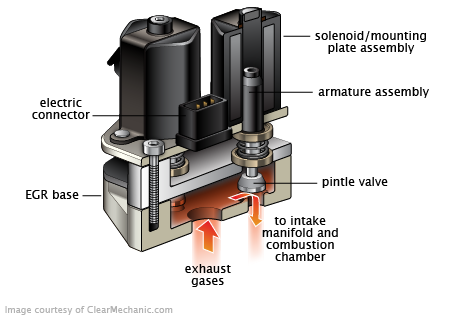
\includegraphics[width=0.75\textwidth]{images/egrvalve.png}
\hfill \url{http://repairpal.com/exhaust-gas-recirculation-system}
\end{center}

\end{frame}

\begin{frame}
\frametitle{Exhaust Gas Recirculator}

Mechanically, the EGR contains a valve which lets exhaust gases back
into the combustion chamber.

\end{frame}

\begin{frame}
\frametitle{Exhaust Gas Recirculator}

First Approach: Fully mechanical system. 

Problem: EGR is not needed in a cold engine.\mnote{When you step on the gas, this opens, and
then closes, the EGR valve. However, you don't need, or want, EGR on a
cold engine, because it lowers the engine's performance. So, GM put a
fully-mechanical thermal switch in its cars. Unfortunately, this
didn't work well, because mechanical components often don't work the
way you want them to, as you'll find out.}

Refinement: More complex mechanical system. \mnote{Car manufacturers added more
components, like vacuum amplifiers, delay valves, and solenoids, to
fix the issues: ``spaghetti'' tubes.}

Problem: more complexity, more cost, more parts that can fail.

Now: Use embedded systems!
\end{frame}

\begin{frame}
\frametitle{Exhaust Gas Recirculator: Inputs \& Outputs}

Inputs: RPM, throttle, temperature (sensors)

Outputs: signal to the valve; pulse-width modulation (actuators)
\end{frame}


\begin{frame}
\frametitle{Exhaust Gas Recirculator: Design Constraints}

\begin{enumerate}
\item Processor power \mnote{The processor must be able to crunch
enough bits. In particular, it needs to have good enough latency (response
time) and bandwidth (processing power) to control the systems it's
responsible for. Plus, you need to be able to model its performance
characteristics.}

\item Environment \mnote{You have to be able to embed the processor. In particular,
you have to respect size, power and connectivity constraints.}
\end{enumerate}
\end{frame}

\begin{frame}
\frametitle{Embedded Systems Challenges}

\begin{itemize}
\item Variability \mnote{Programming Windows systems is all the same, while
programming cellphones is quite different from programming EGRs.}
\item No/bad UI \mnote{Can't necessarily put a print statement into a 
microwave oven's embedded system, nor can you put it in the state
you'd want to.}
\item No API \mnote{An embedded system might not contain any operating system
to speak of.}
\item Hard to get at \mnote{Have to load the software onto the system,
which can be hard.}
\end{itemize}
\end{frame}

\begin{frame}
\frametitle{Plan}

Today we'll look inside a Samsung Galaxy S, with pictures from:

\begin{center}
\url{http://www.ifixit.com/Teardown/Samsung+Galaxy+S+4G+Teardown/4977/1}
\end{center}

\begin{center}
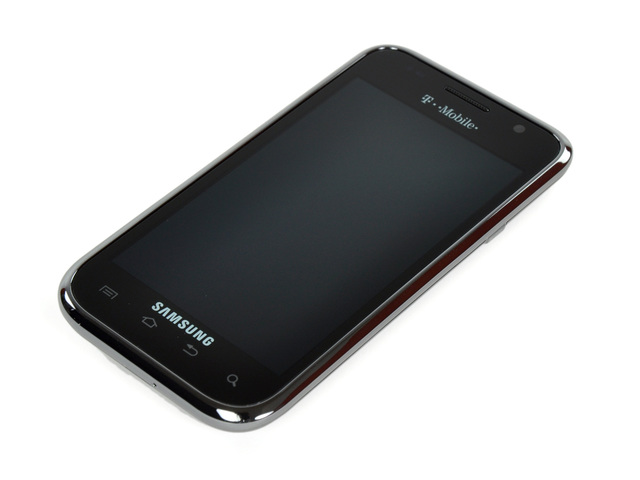
\includegraphics[width=.45\textwidth]{images/GalaxyS4G1-small.jpg}
\end{center}

{\scriptsize Thanks to {\tt ifixit.com} for posting these pictures
under the CC BY-NC-SA license.}

~\\

Educational goal: be able to discuss sensors and actuators, plus embedded operating systems.

\end{frame}

\begin{frame}
\frametitle{Sensors and Actuators}

In particular, today we'll see how a typical phone integrates sensors and
actuators, as typical for embedded systems.
\begin{center}
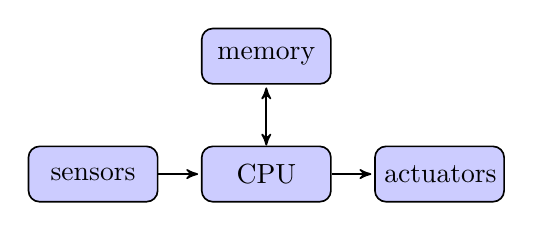
\begin{tikzpicture}[->,>=stealth',shorten >=1pt,auto,node distance=2.2cm,
                    semithick,initial text=]
  \node[bw]   (cpu)               {CPU};
  \node[bw, left of=cpu] (sensors) {sensors};
  \node[bw, right of=cpu] (actuators) {actuators};
  \node[bw, above of=cpu,yshift=-2em] (memory) {memory};

  \path (cpu) edge[<->] node {} (memory)
        (sensors) edge node {} (cpu)
        (cpu) edge node {} (actuators);
\end{tikzpicture}
\end{center}

Specifications:
\begin{itemize}
\item 1GHz ARM ``Hummingbird'' processor\mnote{Cortex A8 processor; nowadays, dual or quad-core processors with A15}\mnote{mention also the big/little concept of modern ARM processor for further power savings}
\item 512MB RAM (plus 1GB storage \& MicroSD slot)
\item 480x800 Super AMOLED display\mnote{display is the biggest energy sink;}
\item 5.0MP and VGA cameras
\end{itemize}
\vspace*{1em}
What actuators can you see?

\end{frame}

\begin{frame}
\frametitle{PCs vs Embedded Systems}

Compare and contrast:

\vspace*{1em}
\scalebox{0.85}{
\begin{tabular}{cc}
\Large PC & \Large \uncover<2->{Embedded System} \\[0.5em]
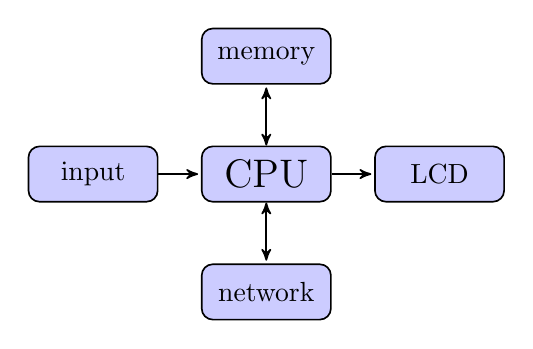
\begin{tikzpicture}[->,>=stealth',shorten >=1pt,auto,node distance=2.2cm,
                    semithick,initial text=]
  \node[bw]   (cpu)               {\Large \alert{CPU}};
  \node[bw, left of=cpu] (sensors) {input};
  \node[bw, right of=cpu] (actuators) {LCD};
  \node[bw, above of=cpu,yshift=-2em] (memory) {memory};
  \node[bw, below of=cpu,yshift=2em] (net) {network};

  \path (cpu) edge[<->] node {} (memory)
        (cpu) edge[<->] node {} (net)
        (sensors) edge node {} (cpu)
        (cpu) edge node {} (actuators);
\end{tikzpicture}
& \uncover<2->{
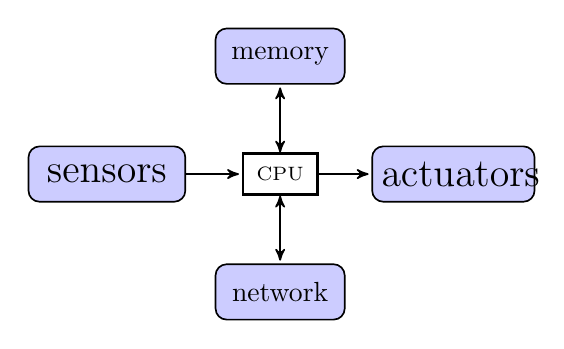
\begin{tikzpicture}[->,>=stealth',shorten >=1pt,auto,node distance=2.2cm,
                    semithick,initial text=]
  \node[block]   (cpu)               {\scriptsize CPU};
  \node[bw, left of=cpu,text width=5em] (sensors) {\Large \alert{sensors}};
  \node[bw, right of=cpu,text width=5.2em] (actuators) {\Large \alert{actuators}};
  \node[bw, above of=cpu,yshift=-2em] (memory) {memory};
  \node[bw, below of=cpu,yshift=2em] (net) {network};

  \path (cpu) edge[<->] node {} (memory)
        (cpu) edge[<->] node {} (net)
        (sensors) edge node {} (cpu)
        (cpu) edge node {} (actuators);
\end{tikzpicture}}
\end{tabular}
}



\end{frame}

\begin{frame}
\frametitle{Opening the Phone}

\begin{center}
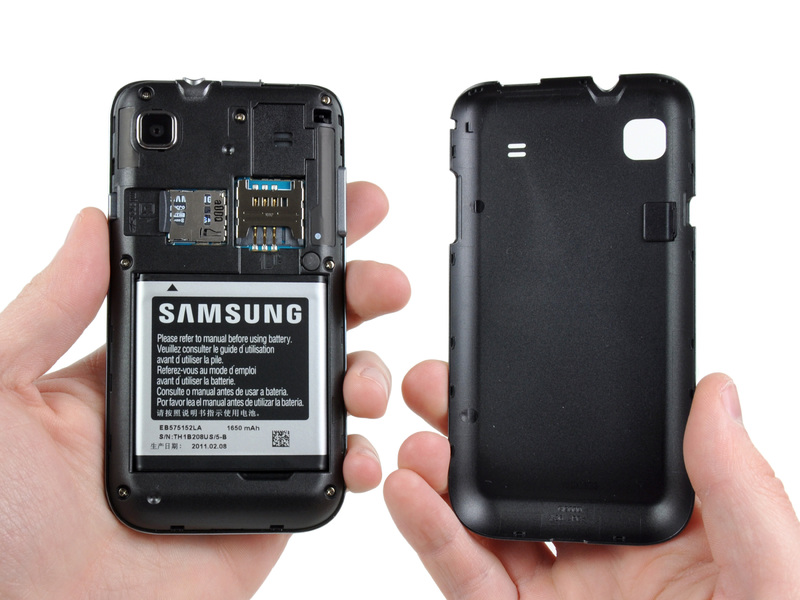
\includegraphics[width=.8\textwidth]{images/GalaxyS4G6-small.jpg}
\end{center}

\end{frame}

\begin{frame}
\frametitle{First Sensors and Actuators}

\begin{center}
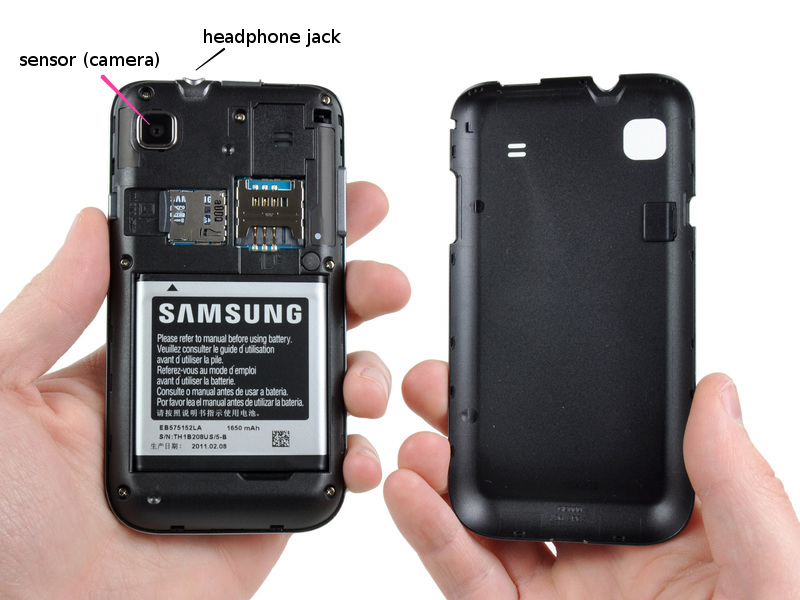
\includegraphics[width=.8\textwidth]{images/GalaxyS4G6-small-annotated.jpg}
\end{center}

\end{frame}

\begin{frame}
\frametitle{Really Opening the Phone}

\vspace*{1em}
This is as far as I'm willing to go with my phone. Thanks, Internet!

\begin{center}
\only<1>{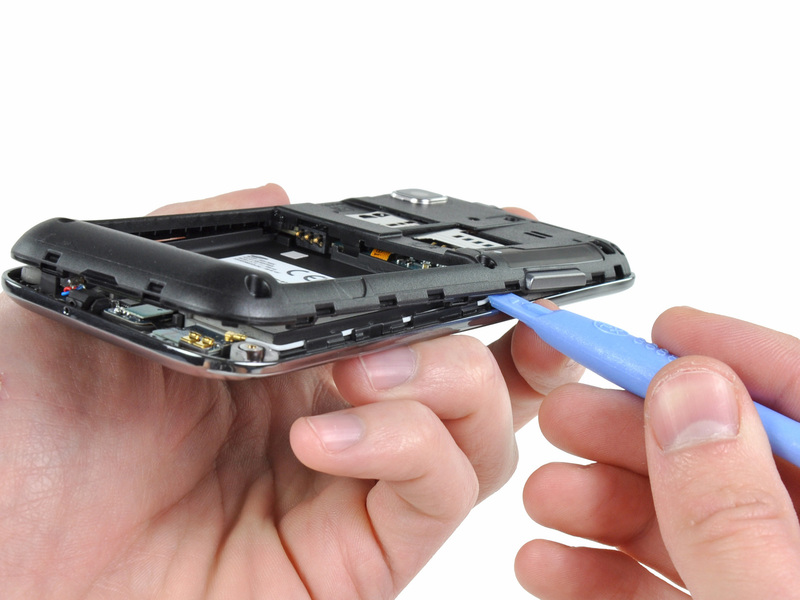
\includegraphics[width=.6\textwidth]{images/GalaxyS4G12-small.jpg}}
\only<2>{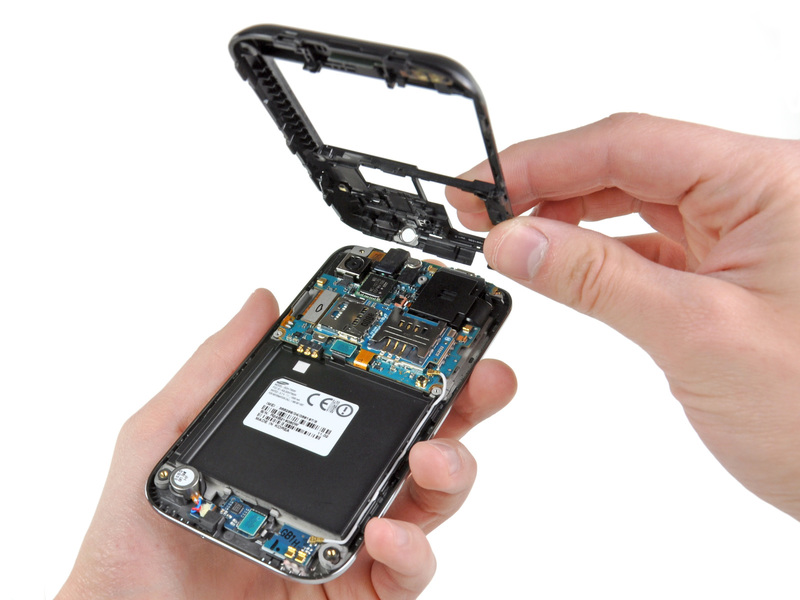
\includegraphics[width=.6\textwidth]{images/GalaxyS4G13-small.jpg}}
\end{center}

We're going to look at the components of the phone now.

\end{frame}

\begin{frame}
\frametitle{Phone Speaker}

\begin{center}
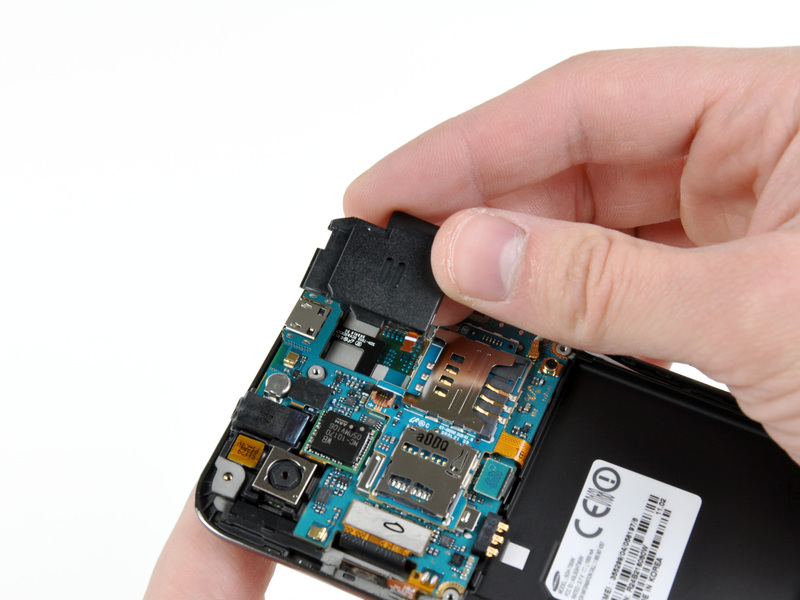
\includegraphics[width=.7\textwidth]{images/GalaxyS4G14-small.jpg}
\end{center}

\hspace*{3em}Speakers are definitely actuators; they move the air.
\begin{center}
\url{http://www.howstuffworks.com/speaker.htm}
\end{center}

\end{frame}

\begin{frame}
\frametitle{Cameras}
\only<1>{\vspace*{3.1em}}
Next up, we have some sensors.

\begin{center}
\only<1>{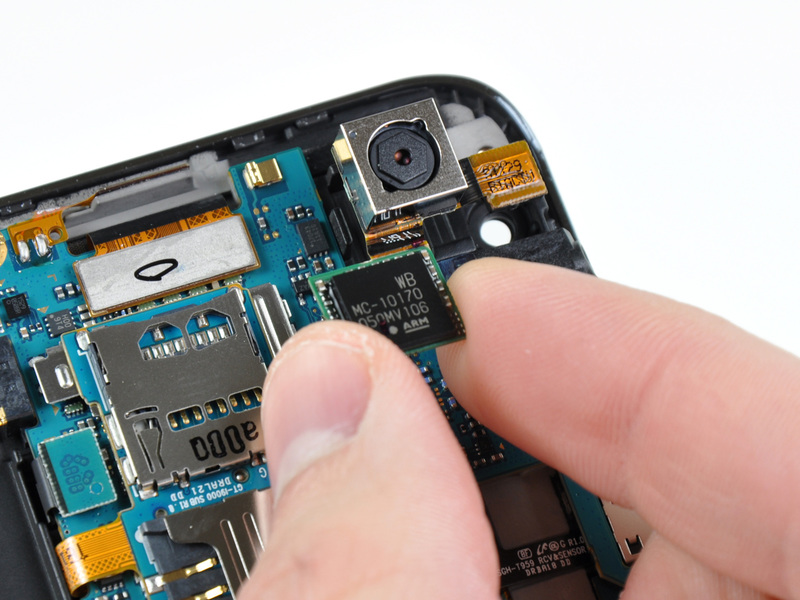
\includegraphics[width=.6\textwidth]{images/GalaxyS4G15-small.jpg}}
\only<2>{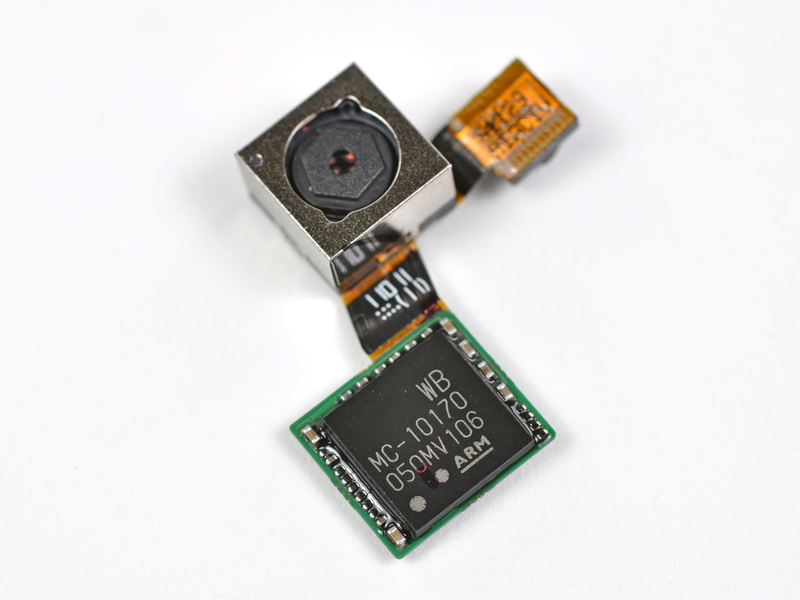
\includegraphics[width=.4\textwidth]{images/GalaxyS4G16-small.jpg}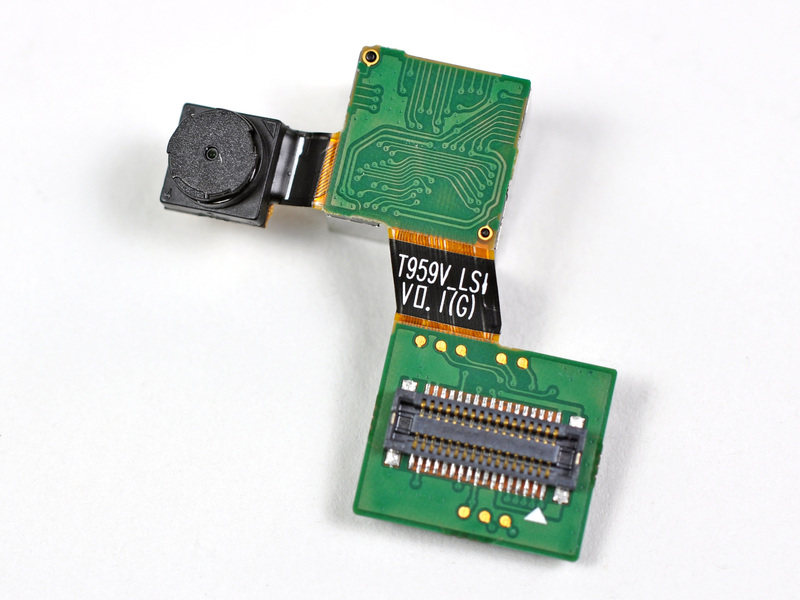
\includegraphics[width=.4\textwidth]{images/GalaxyS4G165-small.jpg}}
\end{center}

\end{frame}

\begin{frame}
\frametitle{The Motherboard}

\begin{center}
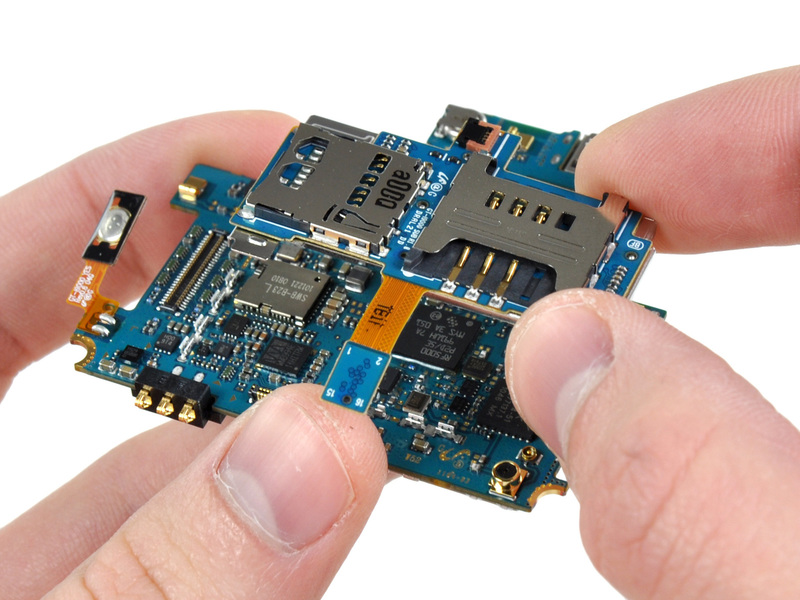
\includegraphics[width=.7\textwidth]{images/GalaxyS4G17-small.jpg}
\end{center}

\mnote{show them the beaglebone board and a raspberry pi board}

\end{frame}

\begin{frame}
\frametitle{Touring the Motherboard Front}

\begin{center}
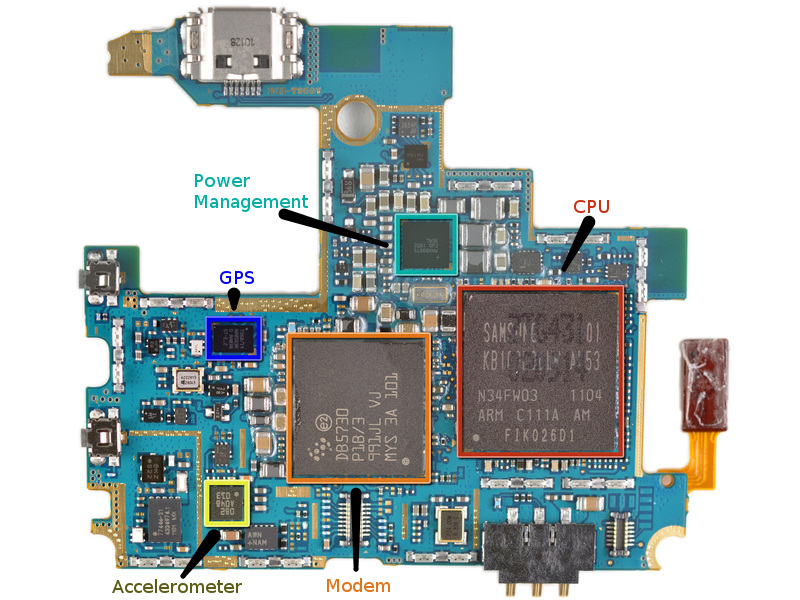
\includegraphics[width=.9\textwidth]{images/Galaxy_Logic_Board_Edited_2_small_annotated.jpg}
\end{center}

\end{frame}

\begin{frame}
\frametitle{Motherboard Back: Mostly Radios}

\begin{center}
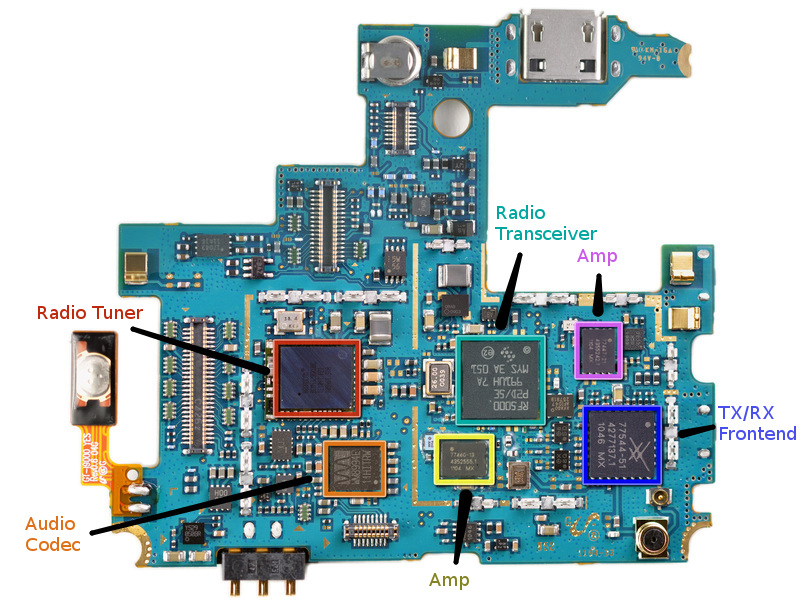
\includegraphics[width=.9\textwidth]{images/Galaxy_Logic_Board_Edited_1_small_annotated.jpg}
\end{center}

\end{frame}

\begin{frame}
\frametitle{Headphone Jack, Earpiece Speaker, Proximity/Light Sensor}
\begin{center}
\only<1>{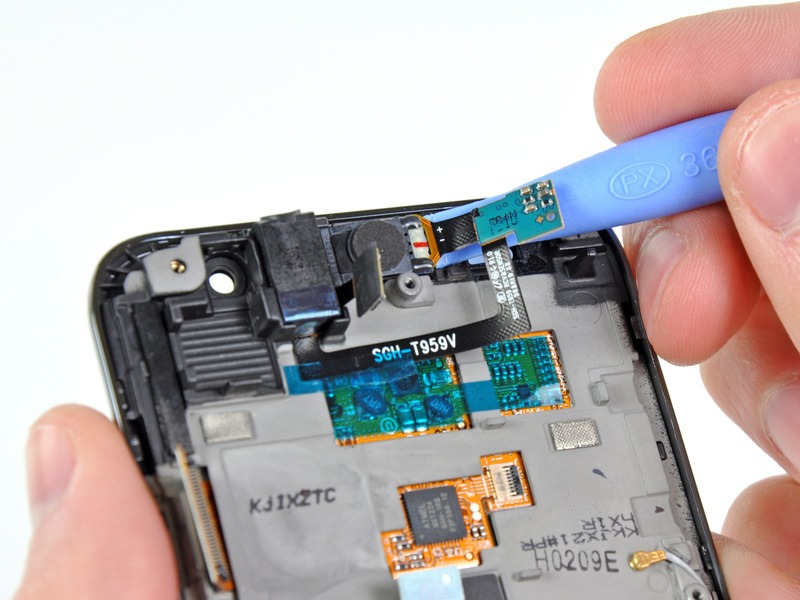
\includegraphics[width=.85\textwidth]{images/Galaxy_S_4G_036-small.jpg}}
\only<2>{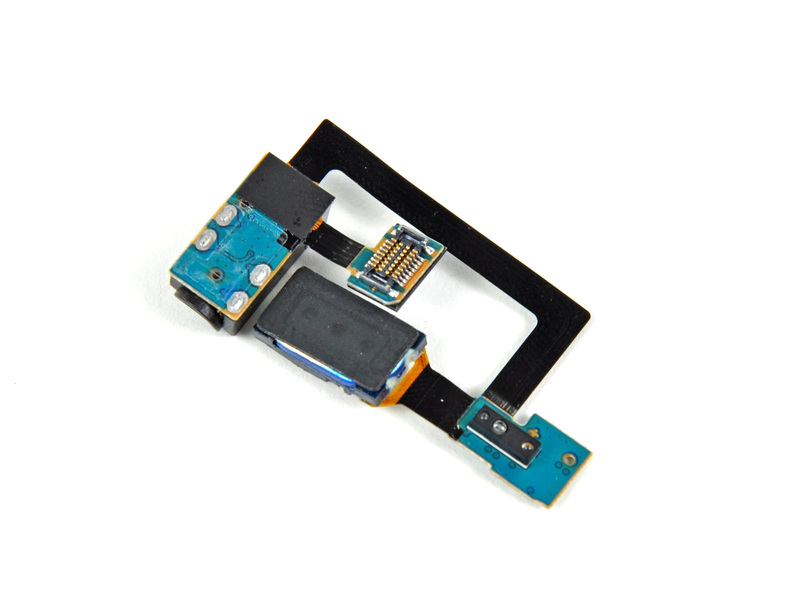
\includegraphics[width=.9\textwidth]{images/Galaxy_S_4G_037-small.jpg}}
\end{center}

\mnote{what's the purpose of the light sensor? to see whether you're holding the phone to your ear. Why is that important? so you don't press buttons with your ear, because it's conductive like your finger.}

\end{frame}


\begin{frame}
\frametitle{Heat Gun!}
\begin{center}
\only<1>{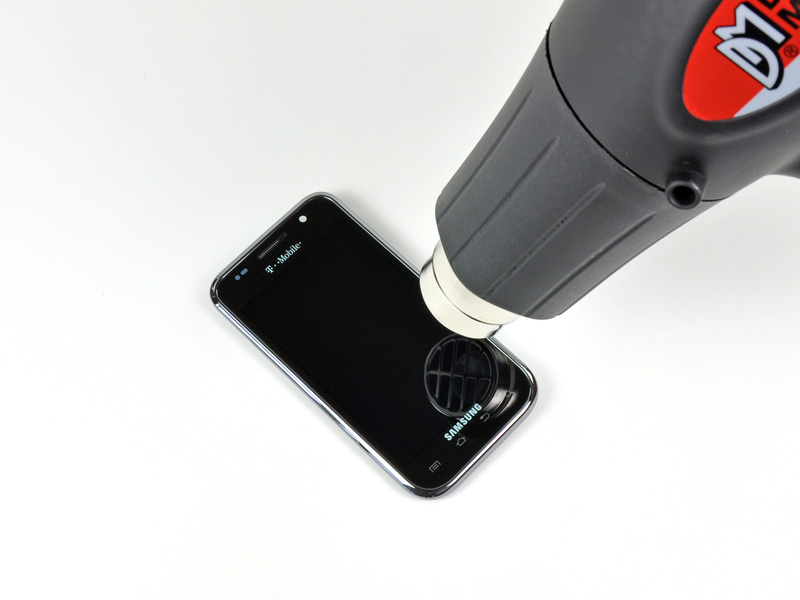
\includegraphics[width=.85\textwidth]{images/Galaxy_S_4G_040-small.jpg}}
\end{center}

\end{frame}

\begin{frame}
\frametitle{Touch Screen Controller}
\begin{center}
\only<1>{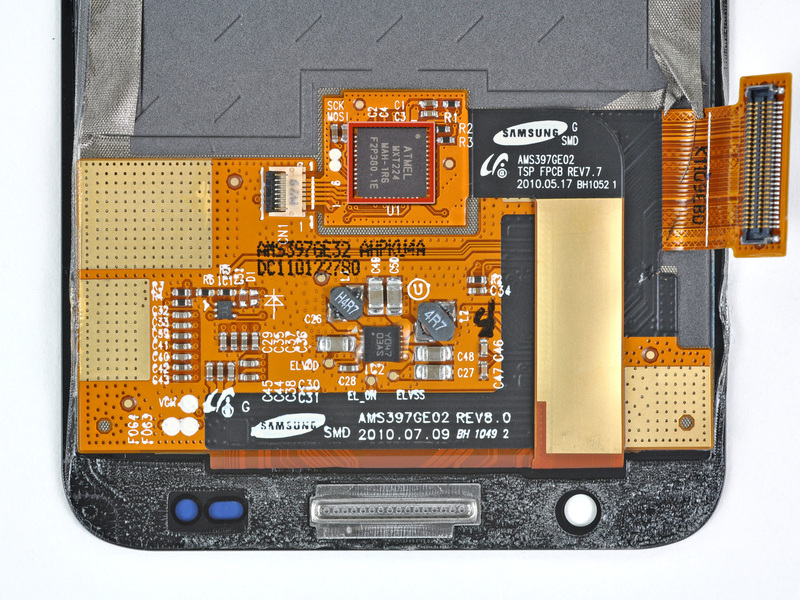
\includegraphics[width=.85\textwidth]{images/Galaxy_S_4G_042-small.jpg}}
\end{center}

\end{frame}

\begin{frame}
\frametitle{Touch Sensors, Vibrator, Microphone, Antenna Cable}
\begin{center}
\only<1>{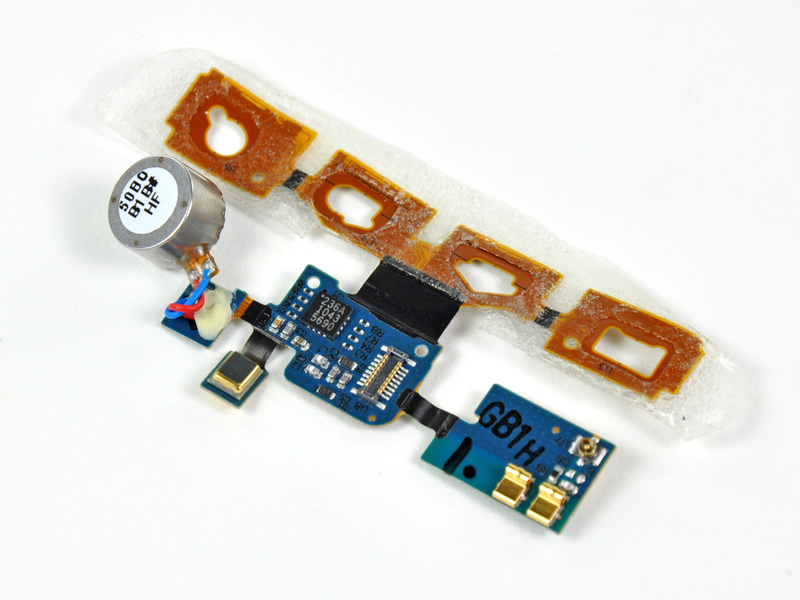
\includegraphics[width=.85\textwidth]{images/Galaxy_S_4G_044-small.jpg}}
\end{center}
\mnote{on modern phones, like the Z10, the touch sensors are integrated into the glass and no longer are a separate layer behind the glass. This is good, because it makes the phone thin, but it can cause costly repairs when the glass breaks}
\end{frame}

\begin{frame}
\frametitle{Summing Up}

\begin{center}
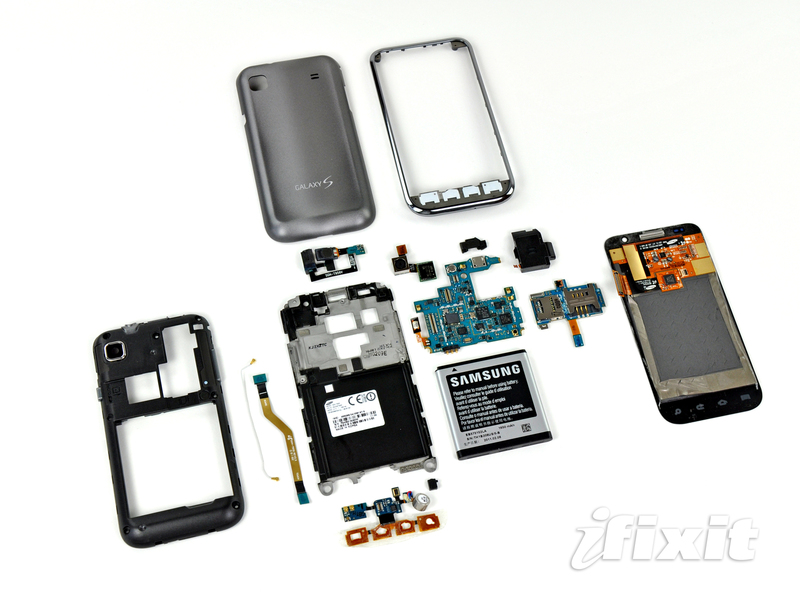
\includegraphics[width=.9\textwidth]{images/Galaxy_S_4G_160-small.jpg}
\end{center}

\end{frame}

\begin{frame}
\frametitle{About Sensors}

Consider a real-world phenomenon (e.g., light intensity):\mnote{ADCs also provide single measurements of input analog voltage into digital value; the x-axis should then just show time}

\begin{center}
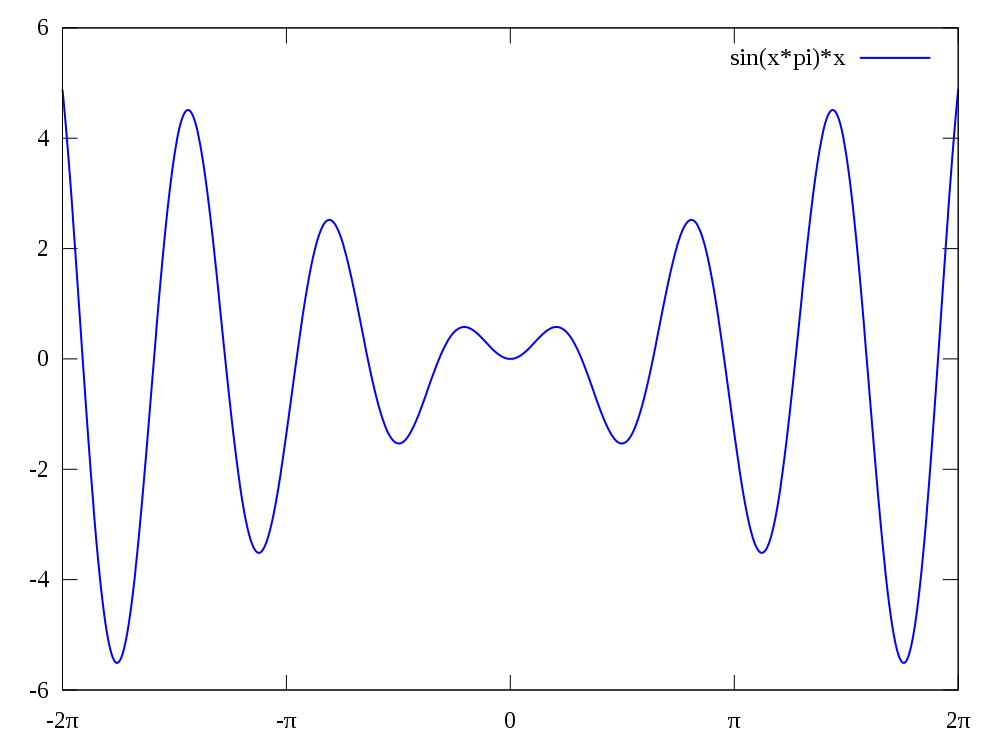
\includegraphics[width=.7\textwidth]{images/sine.png}
\end{center}

Sensor results (in Volts, say) are continuous and analog.

Computers are discrete-time and digital. What to do?
\end{frame}

\begin{frame}
\frametitle{Answer: Sampling}

\mnote{also often called discretization of signals}
\begin{center}
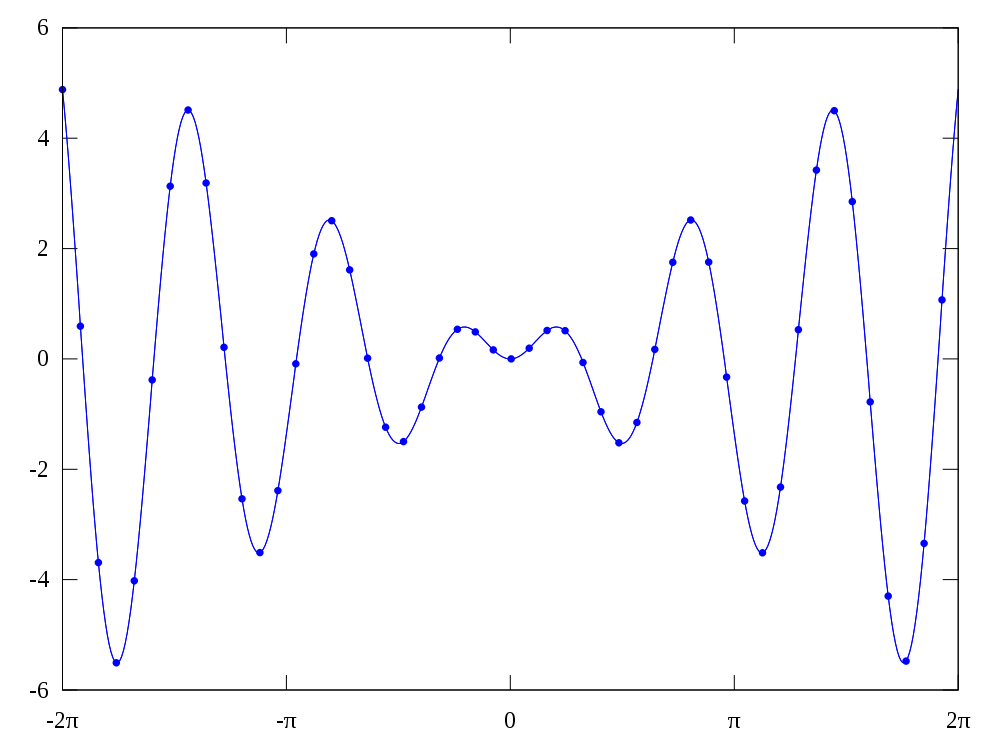
\includegraphics[width=.7\textwidth]{images/sine-points.png}
\end{center}

Report discrete values at given times, e.g.,
\begin{center}$(0, 0), (0.2, 0.12), (0.4, 0.38), (0.6, 0.57), (0.8, 0.47)$.\end{center}

\end{frame}

\begin{frame}
\frametitle{Analog-to-Digital Converter}

\begin{center}
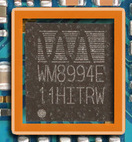
\includegraphics{images/codec.jpg}\\
\hfill (Wolfson Microelectronics WM8994 Audio CODEC)
\end{center}

ADC part of the codec converts continuous-time analog signal to discrete-time
digital signal.\mnote{or show a single measurement of the input voltage; the most frequent use of an ADC for hobbyists when using sensors}

\end{frame}

\begin{frame}
\frametitle{ADC Output}

We lose information if samples too infrequent\footnote{Nyquist sampling theorem.}, or if sample resolution too poor.

\begin{center}
\begin{tabular}{r|r}
Time (ms) & Signal (V) \\ \hline
0.0 & 0.00 \\
0.2 & 0.12 \\
0.4 & 0.38 \\
0.6 & 0.57 \\
0.8 & 0.47 \\
\end{tabular}
\end{center}

~\\[1em]
How would we increase sample frequency? Sample resolution?
\mnote{resolution is controlled by how many bits we have in the decoder; for example 8 bit on a 0-10V system will give you a resolution of 255 steps which is equal to 39 mV}
\end{frame}

\begin{frame}
\frametitle{About Actuators}

Actuators convert output from the computer
system into some effect on the environment. \\[1em]

What are some examples of actuators?\mnote{motors, LCDs, LEDs, heaters/AC units, potentiometer, speakers}\\[4em] 

Some actuators require analog voltage signals;
\begin{itemize}
\item feed the discrete-time data to a digital-to-analog converter
({\bf DAC}).
\end{itemize}

\end{frame}

\begin{frame}
\frametitle{Combined Sensors and Actuators}

\begin{center}
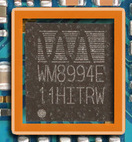
\includegraphics{images/codec.jpg}\\
\hfill (Wolfson Microelectronics WM8994 Audio CODEC)
\end{center}

This contains both an ADC and a DAC.

Also, e.g. piezoelectric sensors are both sensors and actuators.

\end{frame}


\begin{frame}
\frametitle{Programming Embedded Systems}
\begin{center}
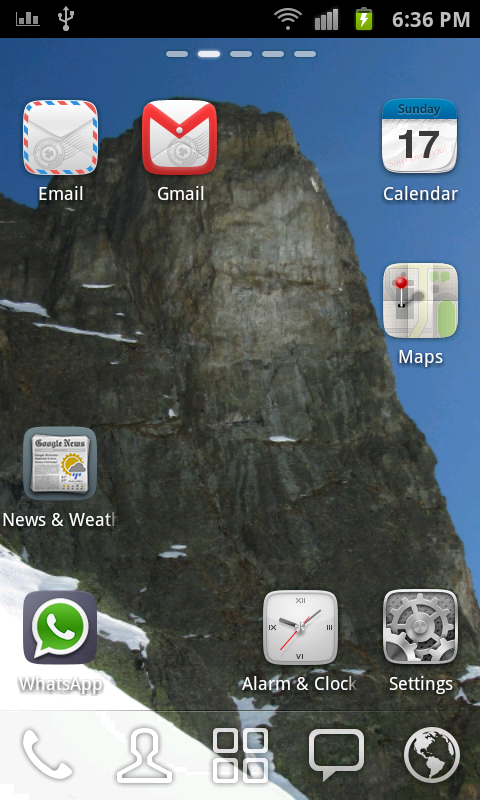
\includegraphics[width=.3\textwidth]{images/android-home}
\end{center}
\hfill --- Android 2.3 embedded operating system.
\end{frame}

\begin{frame}
\frametitle{About Android}

Example of an \alert{embedded operating system}.\\[1em]

Target: smartphones and tablets.
\begin{itemize}
\item Runs Linux under the hood;
\item Using Java, insulates applications from the hardware;
\item Is compact and efficient;
\item Cares about battery life;
\item Favours portability;
\item Available under an open-source license (Apache).
\end{itemize}

We'll learn Android programming in this course.

\end{frame}

\begin{frame}
\frametitle{Lower-level Embedded System Programming}

Consider the modem:

\begin{center}
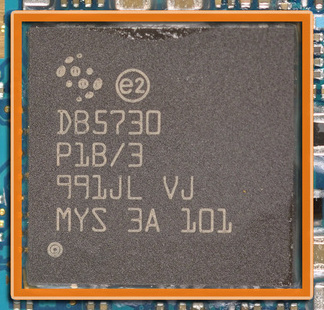
\includegraphics[width=.45\textwidth]{images/modem.jpg}
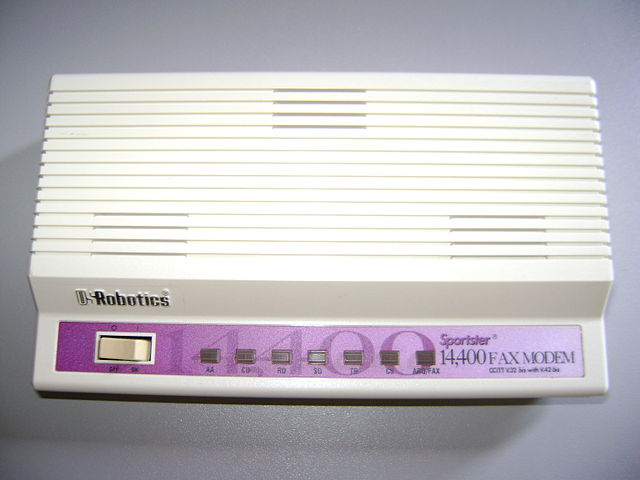
\includegraphics[width=.45\textwidth]{images/640px-Fax_modem_antigo.jpg}\footnote{(credit Wilton Ramon de Carvalho Machado,
\url{http://en.wikipedia.org/wiki/File:Fax_modem_antigo.jpg})}
\end{center}

Converts encoded (radio) signals to and from bits.

\end{frame}

\begin{frame}
\frametitle{Interacting with a Modem}
\begin{center}
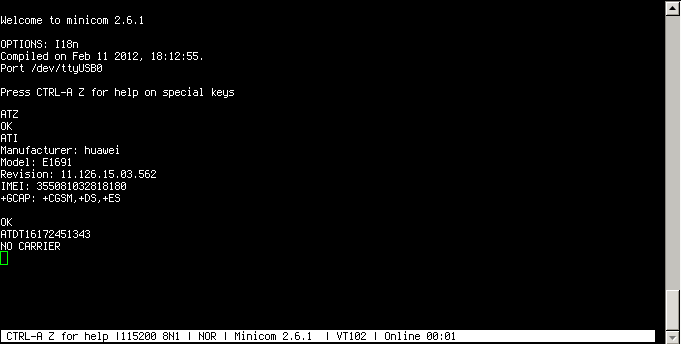
\includegraphics[width=.9\textwidth]{images/modem-interaction.png}
\end{center}

\end{frame}

\begin{frame}
\frametitle{Running an Embedded Control Program}

The modem is running an \alert{embedded control program}.
\begin{itemize}
\item accepts high-level commands from the CPU;
\item translates bits into analog signals; contains an ADC and a DAC.
\end{itemize}

~\\[1em]More generally, the modem:
\begin{itemize}
\item boots automatically;
\item never terminates;
\item translates stream of sensor inputs and actuator outputs;
\item cares about timing.
\end{itemize}
\end{frame}

\begin{multiframe}[Therac-25]
  \begin{center}
    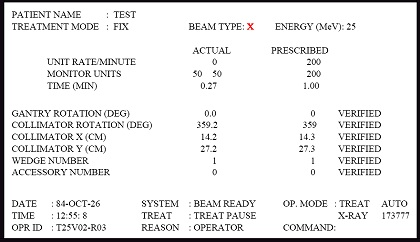
\includegraphics[width=.8\linewidth]{images/Xraybad}
  \end{center}

\end{multiframe} \begin{multiframe}

  \begin{itemize}
  \item Radiation therapy machine
  \item Problem: \alert{many} $\rightarrow$ race conditions, overflow,
    missing safety interlocks
  \item 3 patients died!
  \item Fix: software updates
  \end{itemize}

  \note[item]{\textbf{Problem Race Condition:} Race condition between
    the operator interface task ad the equipment control
    task. Occurred only during quick controlling \textbf{(operator
      practice)}.}

  \note[item]{\textbf{Problem Overflow:} flag was incremented,
    overflow caused software to bypass safety checks.}

  \note[item]{\textbf{Problem Interlocks:} high-energy mode was
    enabled without target in place.}
\end{multiframe}

% --------------------

\begin{frame}[c]
  \frametitle{Conclusion}
  \textbf{\Large Someone has to build these systems!} \\
  Your life will depend on them.

  \pause

   Chances to learn about building safety-critical systems: \\
   \begin{itemize}
   \item ECE455 Embedded Software
   \item SE499: Independent project
   \item FYDP
   \item Undergraduate research assistant
   \end{itemize}
\end{frame}

\begin{frame}
\frametitle{Collaborative Course}

The source material for the ECE~155 notes and slides is now open-sourced via Github. 

If you find an error in the notes/slides, or have an improvement, go to \url{https://github.com/jzarnett/ece155} and open an issue. 

If you know how to use \texttt{git} and \LaTeX, then you can go to the URL and submit a pull request (changes) for me to look at and incorporate!


\end{frame}


\end{document}

